%%%%%%%%%%%%%%%%%%%%%%%%%%%%%%%%%%%%%%%%%%%%%%%%%%%%%%%%%%%%%%%%%%%%%%%%%%%%%%%%%%%%%%%%%%%%%%
%%%%%%%%%%%%%%%%%%%%%%%%%%%%%%%%%%%%%%%%%%%%%%%%%%%%%%%%%%%%%%%%%%%%%%%%%%%%%%%%%%%%%%%%%%%%%%
%%%%%%%%%%% systemOverview
%%%%%%%%%%%%%%%%%%%%%%%%%%%%%%%%%%%%%%%%%%%%%%%%%%%%%%%%%%%%%%%%%%%%%%%%%%%%%%%%%%%%%%%%%%%%%%
%%%%%%%%%%%%%%%%%%%%%%%%%%%%%%%%%%%%%%%%%%%%%%%%%%%%%%%%%%%%%%%%%%%%%%%%%%%%%%%%%%%%%%%%%%%%%%


% \cleardoublepage
\chapter{PAQ Project}
\label{chap:PAQ_project}
Data-aided equalization in aeronautical telemetry has been studied and tested by the Preamble Assisted Equalization (PAQ) project \cite{paq-phase1-report:2014}.
PAQ built a system that compares five data-aided equalizers to blind equalization and no equalization.
Laboratory tests were perfomed using a static RF multipath channel emulator and a noise source to produce Bit Error Rate (BER) curves.
The five data-aided equalizers studied are
\begin{itemize}
\item zero-forcing (ZF) equalizer
\item minimum mean square Error (MMSE) equalizer
\item MMSE-initialized constant modulus algorithm (CMA) equalizer
\item frequency domain equalizer one (FDE1)
\item frequency domain equalizer two (FDE2).
\end{itemize}
Bit error statistics were be used as the figure or merit for the equalization algorithms.
\begin{figure}
	\centering
\includegraphics[width=12.33in/100*50]{figures/intro/received1.pdf}
	\caption{The Received signal has multipath interference, frequency offset, phase offset and additive white Gaussian noise. The received signal is down-converted, filtered, sampled, and resampled to produce the sample sequence $r(n)$.}
	\label{fig:received1}
\end{figure}

\section{System Overview}
The system is summarized by the block diagram in Figure \ref{fig:received1}.
The bit stream $\mathbf{b}$ modulates a SOQPSK-TG carrier.
To enable data-aided equalization, the PAQ bit stream has a packetized structure shown in Figure \ref{fig:packetStructure_intro}.
The bit stream has a pilot bit sequence, in the form of the iNET preamble and ASM, periodically inserted into the data bits.
The iNET preamble comprises eight repetitions of the 16-bit sequence $\text{CD98}_\text{hex}$ and the ASM field is
\begin{equation}
\text{034776C7272895B0}_\text{hex}.
\end{equation}
The data payload is a known length-$(2^{11} - 1)$ PN sequence.
Each packet contains $128$ preamble bits, $64$ ASM bits and $6{,}144$ data bits making each iNET packet $6{,}336$ bits.
The data bit rate is $10$ Mbits/s. 
After preamble and ASM insertion, the bit rate presented to the modulator is $10.3125$ Mbits/s.

After modulation, the transmitted signal experiences multipath interference modeled as an LTI system with the channel impulse response $h(t)$.
The transmitted signal also experiences a frequency offset $\omega_0$, a phase offset $\phi$ and additive white Gaussian noise $w(t)$.
The received signal is down-converted, filtered in the T/M receiver, sampled at $93\nicefrac{1}{3}$ Msamples/second by the ADC, and down-converted to baseband and resampled by $\nicefrac{99}{448}$ in the GPUs in one step using a polyphase filterbank based on the principles outlined in \cite[chap. (9)]{rice:2009}.
The result is $r(n)$, a sampled version of the complex-valued lowpass equivalent waveform at a sample rate of $20.625$ Msamples/second or $2$ samples/bit.
\begin{figure}
	\centering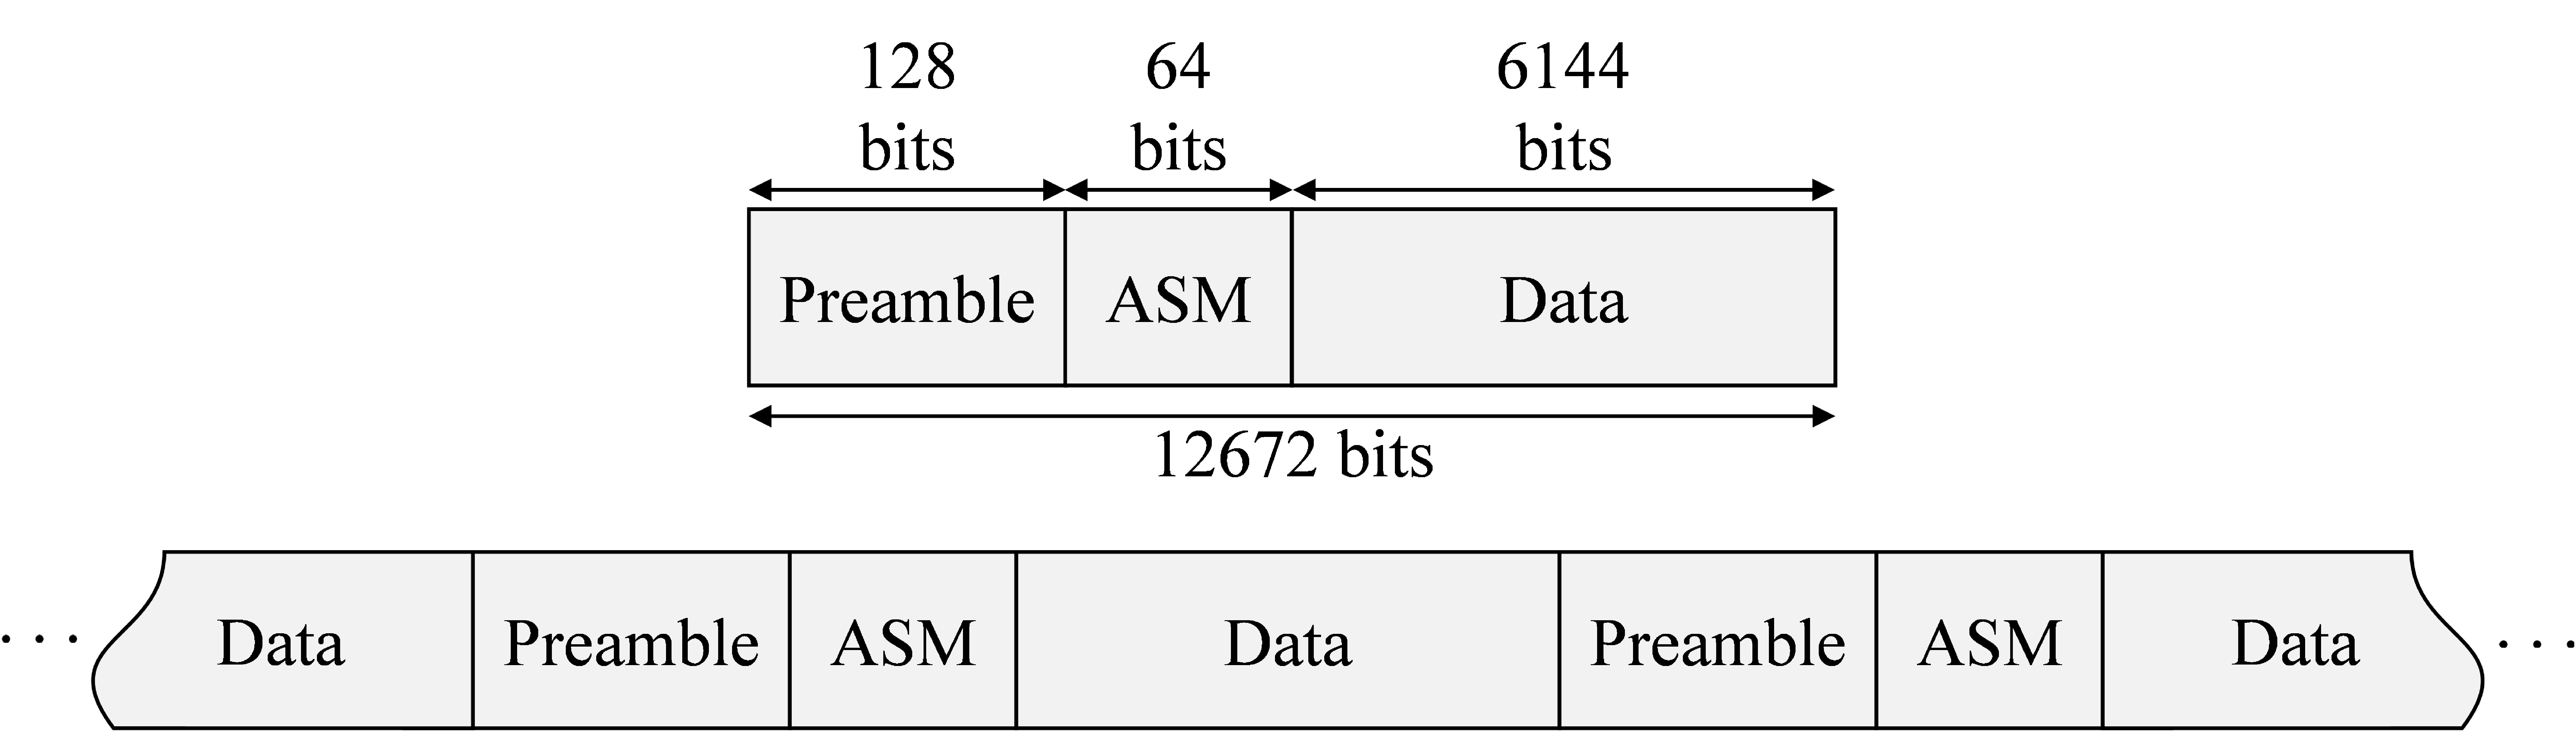
\includegraphics[width=9.47in/100*55]{figures/intro/packetSturcture.pdf}
	\caption{A diagram showing PAQ packetized sample structure.}
	\label{fig:packetStructure_intro}
\end{figure}

\section{Hardware Overview}
\label{sec:hardware}
A block diagram of PAQ physical system is shown in Figure \ref{fig:hardwareblock}.
\begin{figure}
	\centering\includegraphics[width=11.58in/100*55]{figures/systemOverview/hardwareblock.pdf}
	\caption{A block diagram of the physical PAQ hardware. The components inside the rack mounted server are in the dashed box. All the components in the dashed and dotted box are housed in a rack mounted case.}
	\label{fig:hardwareblock}
\end{figure}
A picture of the physical components is shown in Figure \ref{fig:HostSystem}.
\begin{figure}
	\centering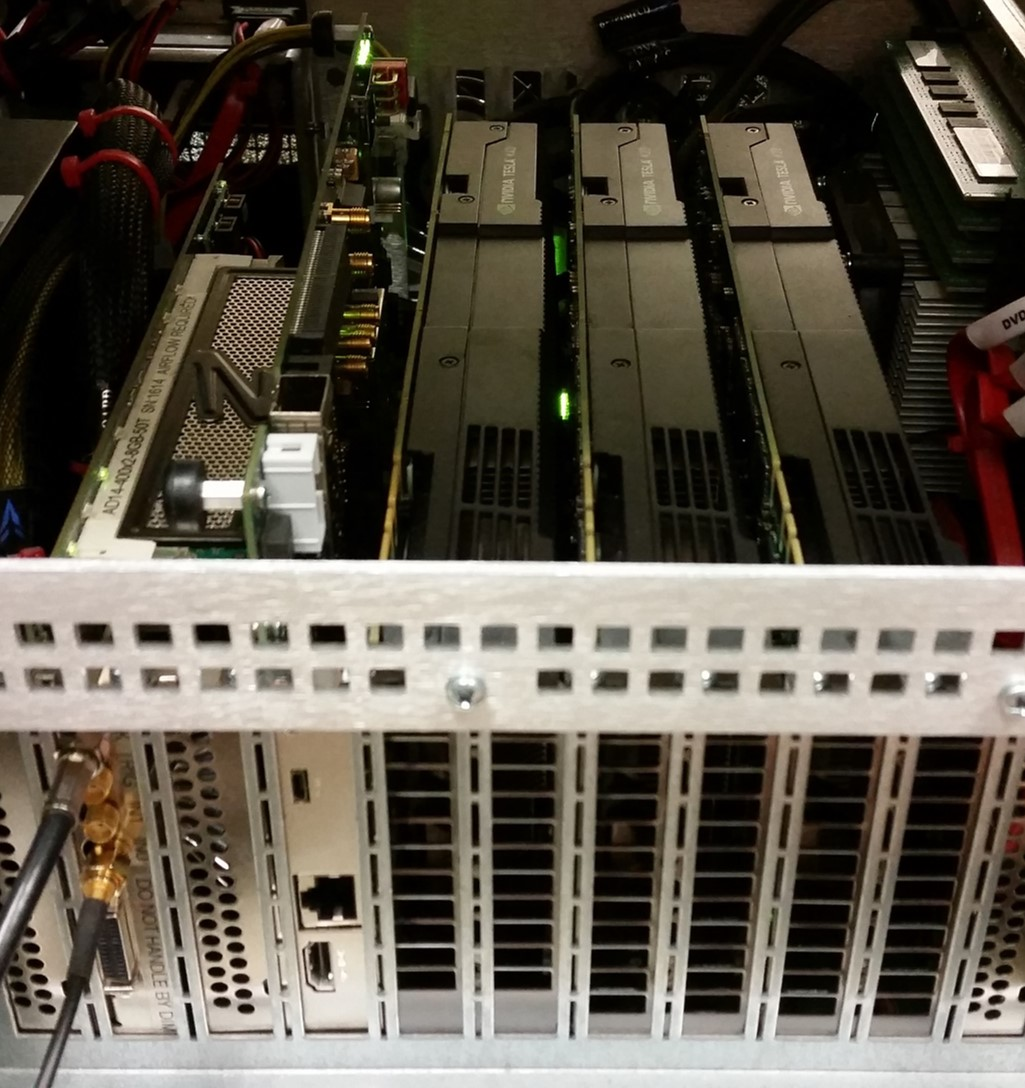
\includegraphics[scale=0.55]{figures/systemOverview/HostSystem.jpg}
	\caption{A picture of the physical PAQ hardware refrencing blocks from Figure \ref{fig:hardwareblock}. Right: Components in the dashed and dotted box. Left: Components in the dashed box. Note that the T/M Receiver is not pictured.}
	\label{fig:HostSystem}
\end{figure}
The major components, and their functions are summarized as follows:
\begin{itemize}
	\item The \textbf{T/M receiver} down-converts the received signal from L- or C-band RF to 70 MHz IF.
	The IF filter plays the role of an anti-aliasing filter.
	%
	\item The \textbf{rack mounted server} is a high powered computer that houses an ADC, a FPGA and three GPUs 		slotted into a 32 pin PCIe bus.
	\item The \textbf{ADC} produces 14-bit samples of the real-valued bandpass IF signal.
	The sample rate is $93\nicefrac{1}{3}$ Msamples/s.
	The samples are transferred to the host CPU via the PCIe bus.
	%
	\item The \textbf{host CPU} initiates memory transfers between itself and the ADC, GPUs and FPGA via the PCIe 	bus. 
	The host CPU also launches the digital signal processing algorithms on the GPUs.
	%
	\item The three \textbf{GPUs} are where the detection, estimation, equalization and demodulation resides.
%	While the CPU has one to eight powerful processors, GPUs have thousands of small less powerful processors that work in parallel. The signal processing is done in GPUs rather than FPGAs or a CPU because programming GPUs is faster and easier than programming FPGAs and CPUs do not prosess the required processing power.
	%
	\item The bit error rate tester (\textbf{BERT}) counts the errors in each bit stream by comparing the 		streams to the transmitted PN sequence.
	%
	\item The \textbf{FPGA} is the interface between the host CPU and the BERT. After the GPUs produce bit decisions, the host CPU transfers the decisions from the GPUs to the FPGA via the PCIe bus. The FPGA then clocks the bits out to the BERT for BER testing.
	%
	\item The \textbf{T/M Receiver \& Demodulator} demodulates the RF signal outputting two bit streams for blind equalization and no equalization for BER comparison.
\end{itemize}
%A picture of the rack mounted physical system is shown in Figure \ref{fig:rack}.
%\begin{figure}
%	\centering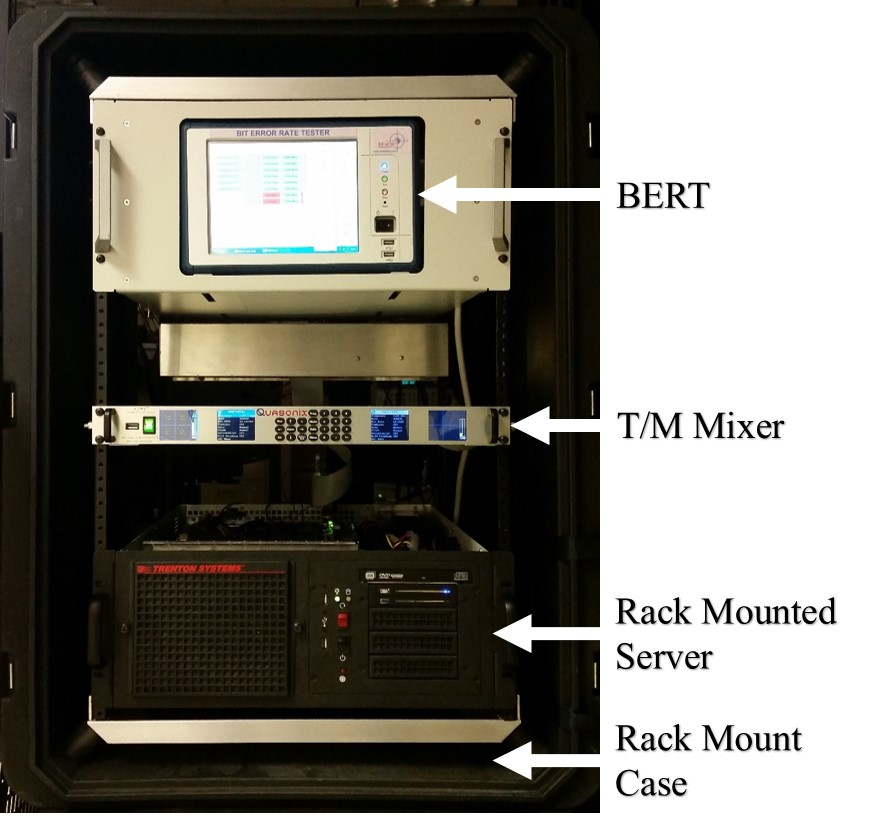
\includegraphics[scale=0.55]{figures/systemOverview/rack.jpg}
%	\caption{A picture of the physical PAQ hardware. Note that the T/M Receiver is not pictured.}
%	\label{fig:rack}
%\end{figure}
%A picture of the components inside the rack mounted server is shown in Figure \ref{fig:rack}.
%\begin{figure}
%	\centering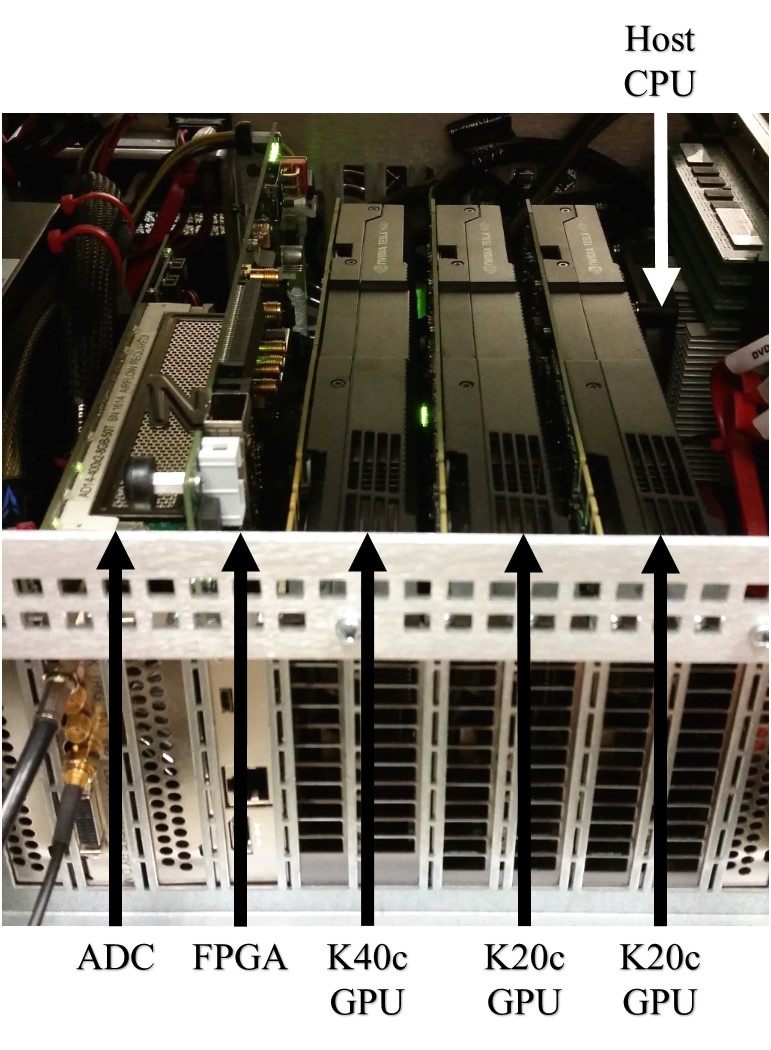
\includegraphics[scale=0.55]{figures/systemOverview/server.jpg}
%	\caption{A pictureof the components inside the rack mounted server.}
%	\label{fig:server}
%\end{figure}

\section{Digital Signal Processing}
\label{sec:signalProcessing}
A high-level digital signal processing flow is shown in Figure \ref{fig:estimators} and \ref{fig:thisThesisBlock}.
The sequence $r(n)$ represents a continuous stream of samples.
Because the frequency offset, channel, and noise variance are estimated using the preamble and ASM, the first step is to find the samples corresponding to the preamble in the received sample sequence $r(n)$.
The preamble detector identifies the sample indices in the sequence $r(n)$ corresponding to the starting position of each occurrence of the waveform samples corresponding to the preamble.
To simplify the notation used to describe the signal processing algorithms, we represent the output of the preamble detector by the vector $\mathbf{r}_\text{p}$, a sequence of $\Lpkt$ samples starting the waveform samples corresponding to the preamble and ASM bits.
In this way the signal processing algorithms are described on a packet-by-packet basis.

Starting with the block diagram of Figure \ref{fig:estimators}, the preamble samples are used first to estimate the frequency offset.
The estimated frequency offset $\hat{\omega}_0$ rads/sample is then used to ``de-rotate'' the vector of samples $\mathbf{r}_\text{p}$ to produce a vector denoted $\mathbf{r}$.
The de-rotated preamble and ASM samples in the vector $\mathbf{r}$ are used to estimate the channel $\hat{\mathbf{h}}$ and noise variance $\hat{\sigma}^2_w$ as shown.
\begin{figure}
	\centering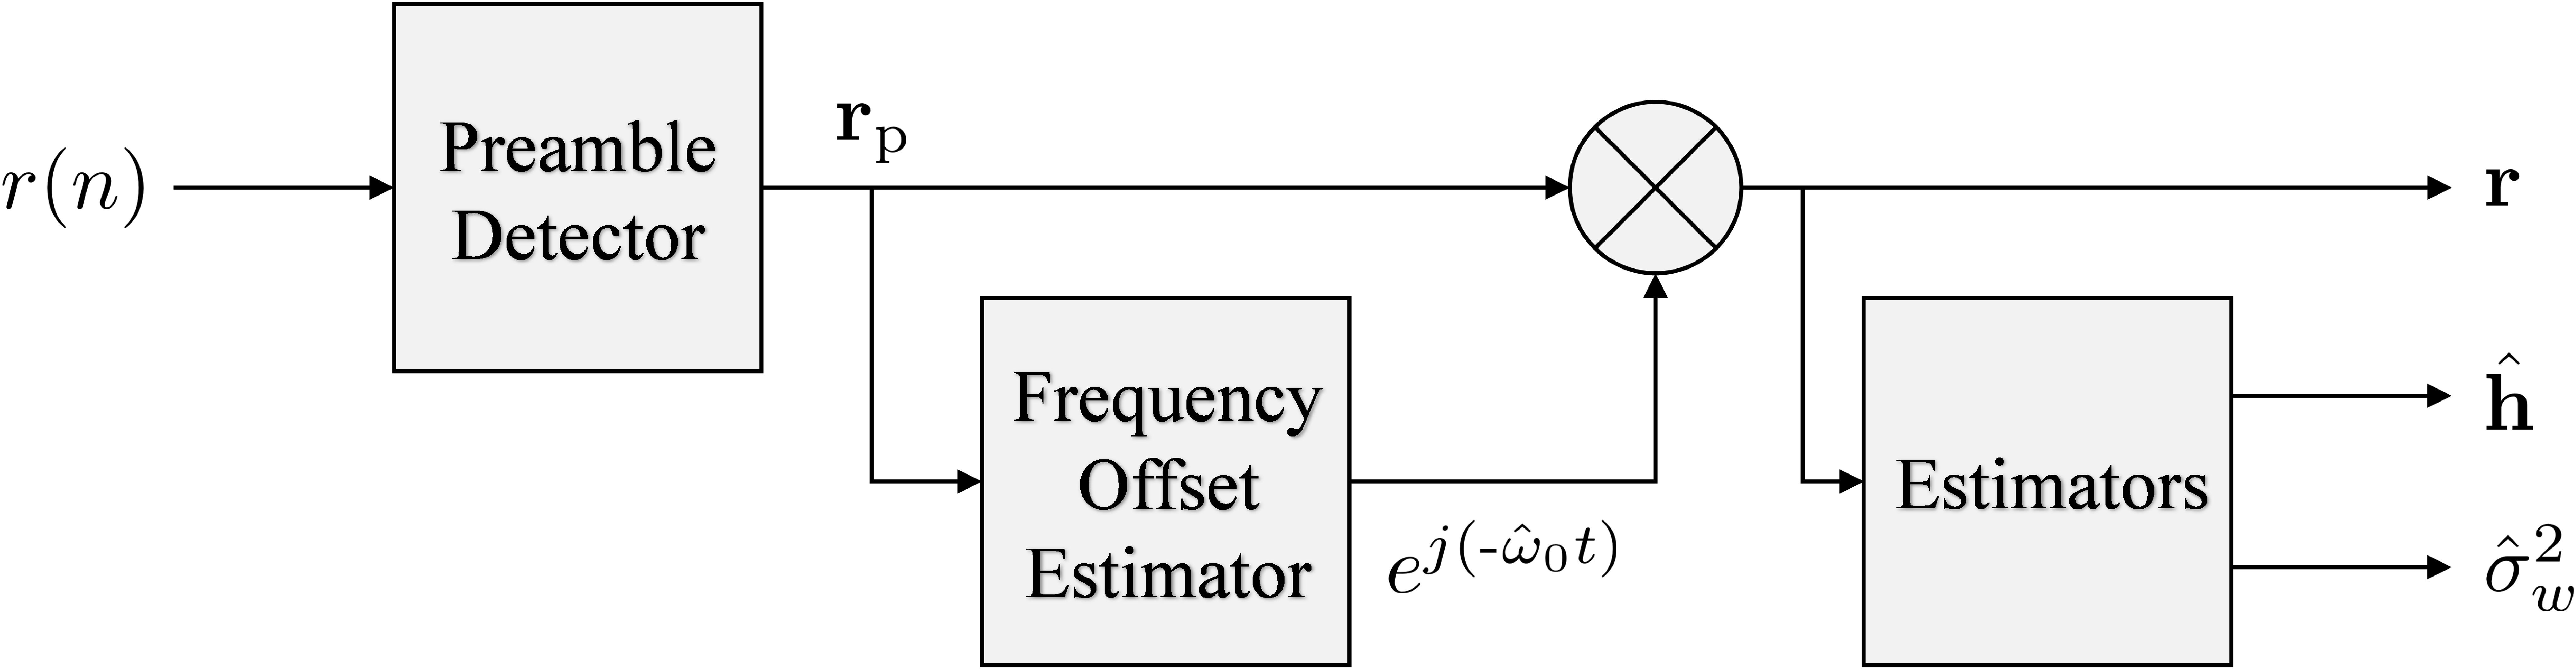
\includegraphics[width=8.75in/100*55]{figures/intro/estimators.pdf}
	\caption{A block diagram of the estimators in PAQ.}
	\label{fig:estimators}
\end{figure}

The estimates produces in Figure \ref{fig:estimators} are used to compute the equalizer filter coefficients as illustrated in Figure \ref{fig:thisThesisBlock}.
The figure shows five independent branches,
each branch computing an equalizer filter.
Lower case boldface $\mathbf{c}$ with a subscript on the top three branches represent impulse responses of the FIR equalizer filters. 
Upper case boldface $\mathbf{C}$ with a on the lower three branches subscript represents the transfer function (FFT) of the equalizer.
In all five cases, the equalizer and a detection filter (described below) are applied to $\mathbf{r}$.
The result is downsampled and processed by a symbol-by-symbol OQPSK detector to produce bit decisions for each equalizer.
\begin{figure}
	\centering\includegraphics[width=10.45in/100*55]{figures/intro/thisThesisBlock5.pdf}
	\caption{A block diagram of the computation and application of the equalizer and detection filters. The bold box emphasizes in the focus of this thesis.}
	\label{fig:thisThesisBlock}
\end{figure}
%\begin{itemize}
%\item The ZF equalizer filter $\mathbf{c}_\text{ZF}$ only requires the channel estimate $\mathbf{\hat{h}}$.
%\item The MMSE equalizer filter $\mathbf{c}_\text{MMSE}$ requires the channel estimate $\mathbf{\hat{h}}$ and the noise variance estimate $\hat{\sigma}^2_w$.
%\item The CMA equalizer filter $\mathbf{c}_\text{CMA}$ requires the de-rotated received signal $\mathbf{r}$ and the MMSE equalizer filter $\mathbf{c}_\text{MMSE}$ for initialization.
%\item The FDE1 equalizer in the frequency domain $\mathbf{C}_\text{FDE1}$ requires the channel estimate $\mathbf{\hat{h}}$ and the noise variance estimate $\hat{\sigma}^2_w$.
%\item The FDE2 equalizer in the frequency domain $\mathbf{C}_\text{FDE2}$ requires the power spectral density of SOQPSK-TG $\mathbf{\Psi}$, the channel estimate $\mathbf{\hat{h}}$ and the noise variance estimate $\hat{\sigma}^2_w$.
%\end{itemize}
%Each branch filters the de-rotated received signal $\mathbf{r}$ with the computed equalizer filter and the detection filter $\mathbf{h}_\text{NO}$.

%The equalizer filters are FIR filters whose impulse response has support $-L_1 \leq n \leq L_2$ (i.e. the equalizer length is $L_\text{EQ} = L_1+L_2+1$ samples).
%The length of the equalizers was batch to five times the length of the channel.
%In particular the non-causal component comprising $L_1 = 5N_1 = 60$ samples and a causal component comprising $L_2 = 5N_2 = 125$ samples resulting in $L_\text{EQ} = L_1+L_2+1 = 186$.
%
%Symbol-by-symbol OQPSK detection \cite[app. (A)]{PAQ-phase1} is performed on the down-sampled equalizer output.
%The $\mathbf{r}_\text{d}$ in each branch has a sample rate of $1$ sample/bit.
%The OQPSK detector block outputs the vector of estimated bits $\hat{\mathbf{b}}$.
%Finally the BER for each equalizer is obtained by comparing the vectors of estimated bits $\hat{\mathbf{b}}$ to the PN sequence.

The GPUs in Figure \ref{fig:hardwareblock} and \ref{fig:HostSystem} perform all the digital signal processing in parallel.
To introduce as much parallelism as possible, the received samples are processed in a batch comprising $39{,}321{,}600$ samples. 
At $20.625$ Msamples/second, each batch of $39{,}321{,}600$ samples represents $1907$ milliseconds of data.
Each batch has at most $3104$ $12{,}672$-sample iNET packets.%
\footnote{Each batch comprises $3103$ or $3104$ packets.}
The GPU processes $3104$ packets in parallel by leveraging batched processing.
To meet the real-time requirement, \textbf{all} processing must be completed in less than $1907$ ms.


This thesis, illustrates how the five PAQ data-aided equalizers were computed and applied in GPUs.
The bold box in Figure \ref{fig:thisThesisBlock} emphasizes processing blocks on which this thesis focuses.
Even though the GPUs process 3104 packets in parallel, the signal processing algorithms are described on a
packet-by-packet basis.

\subsection{Preamble Detection}
\label{sec:pd}
To compute the impulse responses or transfer functions of the five data-aided equalizers, an estimate of the channel and noise variance must be available.
The required estimates are derived from the received waveform samples corresponding to the preamble and ASM bits.
Consequently, the location of the waveform samples corresponding to the preamble and ASM bits must be found.
The preamble detector identifies the sample indices in the sequence $r(n)$ corresponding to the starting position of each occurrence of the waveform samples corresponding to the preamble.
The preamble detector computes the function $L(n)$ for each sample in the batch.
Peaks in $L(n)$ identify the starting indices of the waveform samples corresponding to each occurrence of the preamble bits.
The function $L(n)$ is given by
\begin{equation}
	L(n) = \sum_{m=0}^{7}
		\left[ I^2(n,m) + Q^2(n,m) \right]
	\label{eq:gpu-L-4}
\end{equation}
where
\begin{multline}
	I(n,m) \approx \sum_{\ell\in\mathcal{L}_1}r_R(\ell+32m+n)
			- \sum_{\ell\in\mathcal{L}_2}r_R(\ell+32m+n)
			+ \sum_{\ell\in\mathcal{L}_3}r_I(\ell+32m+n)
			- \sum_{\ell\in\mathcal{L}_4}r_I(\ell+32m+n)
			\\
			+ 0.7071 \left[
				\sum_{\ell\in\mathcal{L}_5}r_R(\ell+32m+n)
				- \sum_{\ell\in\mathcal{L}_6}r_R(\ell+32m+n)
			\right. \\
			\left.
				+ \sum_{\ell\in\mathcal{L}_7}r_I(\ell+32m+n)
				- \sum_{\ell\in\mathcal{L}_8}r_I(\ell+32m+n)
			\right],
	\label{eq:gpu-L-pedone-geoghegan-2}
\end{multline}
and
\begin{multline}
	Q(n,m) \approx \sum_{\ell\in\mathcal{L}_1}r_I(\ell+32m+n)
			- \sum_{\ell\in\mathcal{L}_2}r_I(\ell+32m+n)
			\\
			- \sum_{\ell\in\mathcal{L}_3}r_R(\ell+32m+n)
			+ \sum_{\ell\in\mathcal{L}_4}r_R(\ell+32m+n)
			\\
			+ 0.7071 \left[
				\sum_{\ell\in\mathcal{L}_5}r_I(\ell+32m+n)
				- \sum_{\ell\in\mathcal{L}_6}r_I(\ell+32m+n)
			\right. \\
			\left.
				- \sum_{\ell\in\mathcal{L}_7}r_R(\ell+32m+n)
				+ \sum_{\ell\in\mathcal{L}_8}r_R(\ell+32m+n)
			\right]
		\label{eq:gpu-L-pedone-geoghegan-3}
\end{multline}
with
\begin{equation}
	\begin{split}
	\mathcal{L}_1 &= \{ 0, 8, 16, 24 \}\\
	\mathcal{L}_2 &= \{ 4, 20 \}\\
	\mathcal{L}_3 &= \{ 2, 10, 14, 22 \}\\
	\mathcal{L}_4 &= \{ 6, 18, 26, 30 \}\\
	\mathcal{L}_5 &= \{ 1, 7,  9, 15, 17, 23, 25, 31 \}\\
	\mathcal{L}_6 &= \{ 3, 5, 11, 12, 13, 19, 21, 27, 28, 29 \}\\
	\mathcal{L}_7 &= \{ 1, 3,  9, 11, 12, 13, 15, 21, 23 \}\\
	\mathcal{L}_8 &= \{ 5, 7, 17, 19, 25, 27, 28, 29, 31 \}.
\end{split}
\label{eq:gpu-L-pedone-geoghegan-4}
\end{equation}
A peak in $L(n)$ indicates the index $n$ is the start of a preamble.
Suppose $L(i)$ is a peak (i.e., $i$ is the index of the peak).
The vector $\mathbf{r}_\text{p}$ is 
\begin{equation}
\mathbf{r}_\text{p} = 
\begin{bmatrix}
r(i) \\ 
\vdots \\ 
r(i+\Lpkt-1)
\end{bmatrix}
=
\begin{bmatrix}
r_\text{p}(0) \\ 
\vdots \\ 
r_\text{p}(\Lpkt-1)
\end{bmatrix}
\end{equation}
The first $L_\text{p} = 256$ samples of $\mathbf{r}_\text{p}$ correspond to the preamble bits and the following
$L_\text{ASM} = 128$ samples of $\mathbf{r}_\text{p}$ correspond to the ASM bits.


\subsection{Frequency Offset Compensation}
\label{sec:freq_offset_comp}
The preamble sequence comprises eight copies of the bit sequence CD98\textsubscript{hex}.
Consequently, the waveform samples $r_\text{p}(0), \ldots , r_\text{p}(L_\text{p}-1)$ comprise 
eight copies of $L_q=32$ SOQPSK-TG waveform samples corresponding to CD98\textsubscript{hex}.%
\footnote{This statement is only approximately true. 
Because of the memory in SOQPSK-TG, the first block of $L_q$ is a function of both the bit sequence CD98\textsubscript{hex} and the seven unknown bits preceding the first occurrence of CD98\textsubscript{hex}.}
The frequency offset estimator shown in Figure \ref{fig:estimators} is the estimator taken from \cite[eq. (24)]{rice2014frequency}.
With the notation adjusted slightly, the frequency offset estimate is
\begin{equation}
	\hat{\omega}_0 = \frac{1}{L_q} \arg\left\{ \sum_{n=i+2L_q}^{i+7L_q-1} r_\text{p}(n)r_\text{p}^\ast(n-L_q)\right\}
	\quad
\text{for} \;
i=1,2,3,4,5.
	\label{eq:jeff-ML-w-final3}
\end{equation}
The frequency offset is estimated for every packet or each vector of samples $\mathbf{r}_\text{p}$ in the batch.
Frequency offset compensation is performed by de-rotating the received samples by $-\hat{\omega}_0$:
\begin{equation}
	r(n) = r_\text{p}(n) e^{-j\hat{\omega}_0n}.
	\label{eq:frequency_compensation}
\end{equation}
Equations \eqref{eq:jeff-ML-w-final3} and \eqref{eq:frequency_compensation} are easily implemented into GPUs. 

\subsection{Channel Estimation}
\label{sec:channel_estimation}
Let the SOQPSK-TG samples corresponding to the preamble and ASM bits be
\begin{equation}
\mathbf{p} = 
\begin{bmatrix}
p(0) \\
p(1) \\
\vdots \\
p(L_\text{P} + L_\text{ASM}-1)
\end{bmatrix}.
\label{eq:preamble_ASM}
\end{equation}
The multipath channel is defined by the impulse response 
\begin{equation}
\mathbf{\hat{h}} = 
\begin{bmatrix}
\hat{h}(-N_1) \\ \vdots \\ \hat{h}(0) \\ \vdots \\ \hat{h}(N_2)
\end{bmatrix}.
\end{equation}
Note that at $2$ samples/bit, the complex-valued lowpass equivalent channel impulse response is assumed to have a non-causal component comprising $N_1$ samples and a causal component comprising $N_2$ samples.
Figure \ref{fig:channelExample} shows the full discrete-time $L_h = N_1+N_2+1$ sample channel.
\begin{figure}
	\centering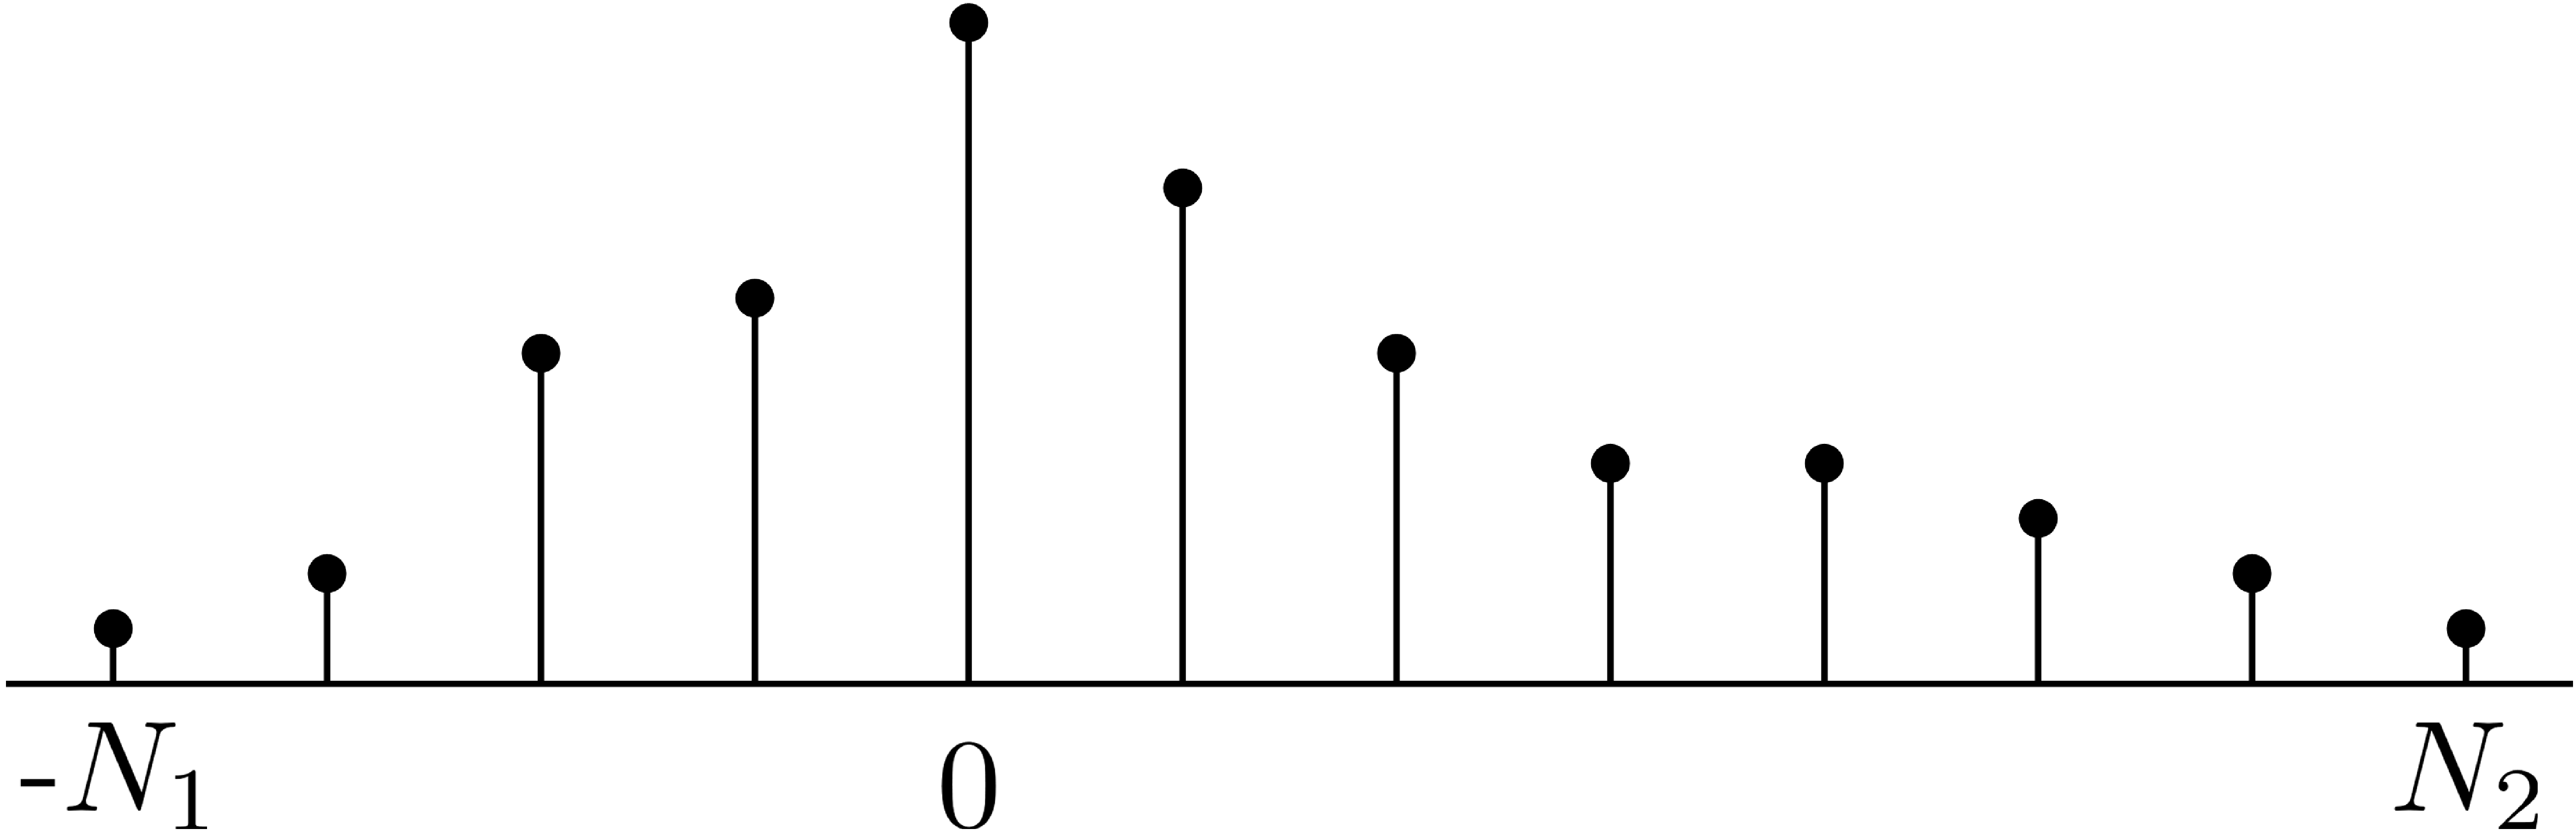
\includegraphics[width=5.5in/100*55]{figures/intro/channelExample.pdf}
	\caption{An illustration of the discrete-time channel of length $N_1+N_2+1$ with a non-causal component comprising $N_1$ samples and a causal component comprising $N_2$ samples.}
	\label{fig:channelExample}
\end{figure}
The ML estimate is \cite[eq. 8]{rice-afran-saquib-cole-rhodes-moazzami:2014} 
\begin{equation}
\hat{\mathbf{h}} = \underbrace{ \left( \mathbf{X}^\dag\mathbf{X} \right)^{-1} \mathbf{X}^\dag}_{\mathbf{X}_\text{lpi}}\mathbf{r}
\end{equation}
where 
\begin{equation}
\mathbf{X} = 
		\begin{bmatrix}
		p(N_2)							& 								& 		&  			\\
		\vdots 							& p(N_2)						& 		&  			\\
		p(L_\text{p}+L_\text{ASM}-N_1)	&\vdots							& \ddots&  			\\
										& p(L_\text{p}+L_\text{ASM}-N_1)&  		& p(N_2)  	\\
		 								&  								&  		& \vdots 	\\
		 								&  	   							&  		& p(L_\text{p}+L_\text{ASM}-N_1)\\
	\end{bmatrix}
	\label{eq:X}
\end{equation}
is the $(L_\text{p}+L_\text{ASM}-N_1-N_2)\times(N_1+N_2+1)$ convolution matrix formed from 
the SOQPSK-TG waveform samples corresponding to the preamble and ASM bits.
The $(N_1+N_2+1)\times(L_\text{p}+L_\text{ASM}-N_1-N_2)$ matrix $\mathbf{X}_\text{lpi}$ is the left pseudo-inverse of $\mathbf{X}$.
The matrix vector multiplication $\mathbf{X}_\text{lpi} \mathbf{r}$ is implemented simply and efficiently in GPUs.


\subsection{Noise Variance Estimation}
\label{sec:noise_variance_estimation}
The noise variance estimator is \cite[eq. 9]{rice-afran-saquib-cole-rhodes-moazzami:2014}
\begin{equation}
	\hat{\sigma}_w^2 = \frac{1}{2\rho} \left| \mathbf{r}-\mathbf{X}\hat{\mathbf{h}}\right|^2
	\label{eq:ML-s2-final3}
\end{equation}
where
\begin{equation}
	\rho = {\rm Trace} \left\{ \mathbf{I} -  \mathbf{X}\left(\mathbf{X}^\dag\mathbf{X}\right)^{-1}\mathbf{X}^\dag \right\}
\end{equation}
where $\mathbf{X}$ is given by Equation \eqref{eq:X}.
Equation \eqref{eq:ML-s2-final3} is easily implemented into GPUs.

\subsection{Equalizers}

\subsubsection{Zero-Forcing Equalizer}
The ZF equalizer is an FIR filter defined by the $L_\text{eq}=L_1+L_2+1$ coefficients
\begin{equation}
\mathbf{c}_\text{ZF} = 
\begin{bmatrix}
c_\text{ZF}(-L_1) \\ \vdots \\ c_\text{ZF}(0) \\ \vdots \\ c_\text{ZF}(L_2).
\end{bmatrix}.
\end{equation}
The filter coefficients are the solution to \cite{paq-phase1-report:2014}
\begin{equation}
\mathbf{R}_{\hat{h}} \mathbf{c}_\text{ZF} = \hat{\mathbf{g}}
\label{eq:start_here_ZF_MDR}
\end{equation}
where
\begin{equation}
\mathbf{R}_{\hat{h}} = 
		\begin{bmatrix}
		r_{\hat{h}}(0)			& r^\ast_{\hat{h}}(1)	& \cdots 	& r^\ast_{\hat{h}}(L_{eq}-1)  	\\
		r_{\hat{h}}(1) 			& r_{\hat{h}}(0)		& \cdots 	& r^\ast_{\hat{h}}(L_{eq}-2)  	\\
		\vdots	 				& \vdots				& \ddots 	&  								\\
		r_{\hat{h}}(L_{eq}-1)	& r_{\hat{h}}(L_{eq}-2)	& \cdots	& r_{\hat{h}}(0)  			
	\end{bmatrix},
	\label{eq:R_h_MDR}
\end{equation}
\begin{equation}
\hat{\mathbf{g}} = 
\begin{bmatrix} \hat{h}^\ast(L_1) \\ \vdots \\ \hat{h}^\ast(0) \\ \vdots \\ \hat{h}^\ast(-L_2)  \end{bmatrix},
\label{eq:g_MDR}
\end{equation}
and
\begin{equation}
r_{\hat{h}}(k) = \sum_{n=-N_1}^{N_2} \hat{h}(n) \hat{h}^\ast(n-k),
\label{eq:sample_autocorrelation_ZF_MDR}
\end{equation}

\subsubsection{MMSE Equalizer}
The MMSE equalizer is an FIR filter defined by the $L_\text{eq}=L_1+L_2+1$ coefficients
\begin{equation}
\mathbf{c}_\text{MMSE} = 
\begin{bmatrix}
c_\text{MMSE}(-L_1) \\ \vdots \\ c_\text{MMSE}(0) \\ \vdots \\ c_\text{MMSE}(L_2).
\end{bmatrix}.
\end{equation}
The filter coefficients are the solution to \cite{paq-phase1-report:2014}
\begin{equation}
\mathbf{R} \mathbf{c}_\text{MMSE} = \hat{\mathbf{g}}
\label{eq:start_here_MMSE_MDR}
\end{equation}
where
\begin{equation}
\mathbf{R} = 
\mathbf{R}_{\hat{\mathbf{h}}} + \hat{\sigma}^2_w \mathbf{I},
\end{equation}
$\mathbf{R}_{\hat{\mathbf{h}}}$ is given by \eqref{eq:R_h_MDR}, $\hat{\sigma}^2_w$ is given by \eqref{eq:ML-s2-final3}, and $\hat{\mathbf{g}}$ is given by \eqref{eq:g_MDR}.

\subsubsection{Constant Modulus Algorithm Equalizer}
The CMA equalizer is an adaptive FIR filter where the $L_\text{eq}=L_1+L_2+1$ coefficients at the $b$-th iteration are
\begin{equation}
\mathbf{c}_\text{CMA}^{(b)} = 
\begin{bmatrix}
c_\text{CMA}^{(b)}(-L_1) \\ \vdots \\ c_\text{CMA}^{(b)}(0) \\ \vdots \\ c_\text{CMA}^{(b)}(L_2).
\end{bmatrix}.
\end{equation}
The equalizer output at the $b$-th iteration is 
\begin{equation}
\mathbf{y}^{(b)} = 
\mathbf{c}_\text{CMA}^{(b)} \ast \mathbf{r}.
\end{equation}
Note that in this implementation the CMA filter coefficients are constant for the duration of a packet \cite{rice-afran-saquib-cole-rhodes-moazzami:2014}.
The filter coefficients are updated on a packet-by-packet basis using a steepest descent algorithm as follows:
\begin{equation}
\mathbf{c}_\text{CMA}^{(b+1)} = \mathbf{c}_\text{CMA}^{{b}}-\mu \nabla J
\label{eq:steepest}
\end{equation}
where
\begin{equation}
	\nabla J = \frac{2}{L_{pkt}} \sum_{n=0}^{L_{pkt}-1}
	\left[ \vphantom{\displaystyle\sum}  y^{(b)}(n) \left( y^{(b)}(n)\right)^\ast - 1 \right]
	y^{(b)}(n)  \mathbf{r}^\ast(n).
\label{eq:DelJcma-approxr_MDR}
\end{equation}
In Equation \eqref{eq:DelJcma-approxr_MDR}, $y^{(b)}(n)$ is the $n$-th element of the vector $\mathbf{y}^{(b)}$ and
\begin{equation}
\mathbf{r}(n) = \begin{bmatrix} r(n+L_1) \\ \vdots \\ r(n) \\ \vdots \\ r(n-L_2) \end{bmatrix}.
\end{equation}

\subsubsection{Frequency Domain Equalizer One}
Frequency-domain equalization leverages the efficiency of the FFT algorithm to perform equalization filtering in the FFT domain.
The difference between frequency-domain equalization and applying the previous three equalizer filters in the FFT domain is that the frequency-domain equalizer is computed directly in the FFT domain.
To enable this, some provision must be made for the fact that point-by-point multiplication in the FFT domain corresponds to \textit{circular} convolution in the time domain.
This provision is most often in the form of a cyclic prefix prepended to the data packet \cite{sari1994frequency,ng2007turbo,al2008single,proakis-salehi:2008}.
Even though the PAQ format does not include any special provision for frequency-domain equalization such as a cyclic prefix, frequency-domain equalization is still possible using the ideas described by Coon et al \cite{coon-sandell-beach-mcgeehan:2006}.
Because of the repetitive nature of the preamble sequence, the second half of the preamble bits at the beginning of the packet are the same the first half of the preamble bits following the packet.
Consequently, the second half of the preamble bits at the beginning of the packet form a cyclic prefix for the block comprising the ASM, the data, and the first half of the preamble following the packet as illustrated in Figure \ref{fig:cyclicPrefix_MDR}.
\begin{figure}
	\centering\includegraphics[width=9.47in/100*55]{figures/eq_equations/cyclicPrefix.pdf}
	\caption{A diagram showing how the iNET packet is used as a cyclic prefix.}
	\label{fig:cyclicPrefix_MDR}
\end{figure}

The FFT domain transfer function of FDE1 is \cite[eq. (11)]{williams2013linear}
\begin{equation}
C_\text{FDE1}(e^{j\omega_k}) = \frac{\hat{H}^\ast(e^{j\omega_k})}  {|\hat{H}(e^{j\omega_k})|^2  +  \frac{1}{\hat{\sigma}^2_w}} \quad
\omega_k = \frac{2\pi}{N_\text{FFT}} \;
\text{for} \;
k=0,1,\cdots,N_\text{FFT}-1
\label{eq:FDE1_MDR}
\end{equation}
where $N_\text{FFT} = 2^u = 16{,}384$, where $u = {\left\lceil \log_2{\left(\Lpkt\right)}  \right\rceil} = 14$,
where $\left\lceil x  \right\rceil$ means the smallest integer greater than or equal to $x$.
In Equation \eqref{eq:FDE1_MDR}, $\hat{H}(e^{j\omega_k})$ is the $k$-th element of the length-$N_\text{FFT}$ FFT of $\mathbf{\hat{h}}$ and $\hat{\sigma}^2$ is given by \eqref{eq:ML-s2-final3}.
FDE1 is the MMSE equalizer formulated in the frequency domain where power spectral density of SOQPSK-TG is a constant.

\subsubsection{Frequency Domain Equalizer Two}
The FFT domain transfer function of FDE1 is \cite[eq. (12)]{williams2013linear}
\begin{equation}
C_\text{FDE2}(e^{j\omega_k}) = \frac{\hat{H}^\ast(e^{j\omega_k})}  {|\hat{H}(e^{j\omega_k})|^2  +  \frac{\Psi(e^{j\omega_k})}{\hat{\sigma}^2_w}} \quad
\omega_k = \frac{2\pi}{N_\text{FFT}} \;
\text{for} \;
k=0,1,\cdots,N_\text{FFT}-1
\label{eq:FDE2_MDR}
\end{equation}
where $N_\text{FFT} = 2^u = 16{,}384$, where $u = {\left\lceil \log_2{\left(\Lpkt\right)}  \right\rceil} = 14$,
where $\left\lceil x  \right\rceil$ means the smallest integer greater than or equal to $x$.
In Equation \eqref{eq:FDE2_MDR}, $\hat{H}(e^{j\omega_k})$ is the $k$-th element of the length-$N_\text{FFT}$ FFT of $\mathbf{\hat{h}}$ and $\hat{\sigma}^2$ is given by \eqref{eq:ML-s2-final3}.
Like FDE1, FDE2 is the MMSE equalizer formulated in the frequency domain.
The difference is FDE2 uses an estimate of the true power spectral density of SOQPSK-TG.
The SOQPSK-TG power spectral density $\Psi(e^{j\omega_k})$ is illustrated in Figure \ref{fig:SOQPSK_spectrum_MDR}.
$\Psi(e^{j\omega_k})$ was estimated using Welch's method periodogram averaging based on length-$N_\text{FFT} $ FFTs of SOQPSK-TG sampled at $2$ samples/bit and the Blackman window with $50\%$ overlap.
\begin{figure}
	\centering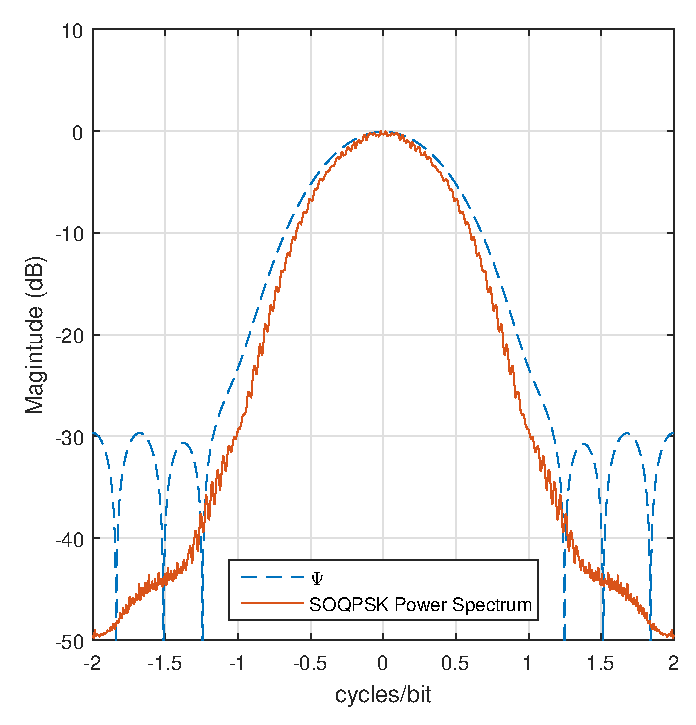
\includegraphics[width=5in]{figures/eq_equations/FDE2_spectrum_PSI.eps}
	\caption{SOQPSK-TG power spectral density.}
	\label{fig:SOQPSK_spectrum_MDR}
\end{figure}

\subsection{Symbol-by-Symbol Detector}
\label{sec:oqpsk_detector}
Symbol-by-symbol detection comprises a detection filter and a phase lock loop (PLL) to track out the residual frequency offset.
Before the symbols are detected, the equalized samples are passed through the detection filter then down-sampled by $2$. 
The detection filter is a $L_\text{df} = 23$ sample ``numerically optimized'' SOQPSK detection filter $\mathbf{h}_\text{NO}$ shown in Figure \ref{fig:detectionFilter}
\cite[Fig. 3]{perrins:2013}.
\begin{figure}
	\centering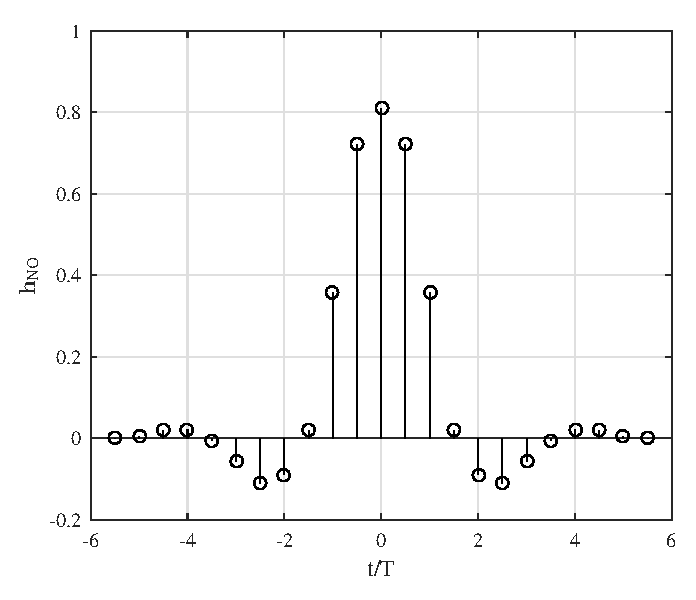
\includegraphics[width=5in]{figures/eq_equations/df.eps}
	\caption{``Numerically optimized'' SOQPSK detection filter $\mathbf{h}_\text{NO}$.}
	\label{fig:detectionFilter}
\end{figure}
The symbol-by-symbol detector block in Figure \ref{fig:thisThesisBlock} is an OQPSK detector.
Using the simple OQPSK detector in place of a complex MLSE SOQPSK-TG detector leads to less than $1$ dB loss in detection efficency \cite{perrins:2013}.
\begin{figure}
	\centering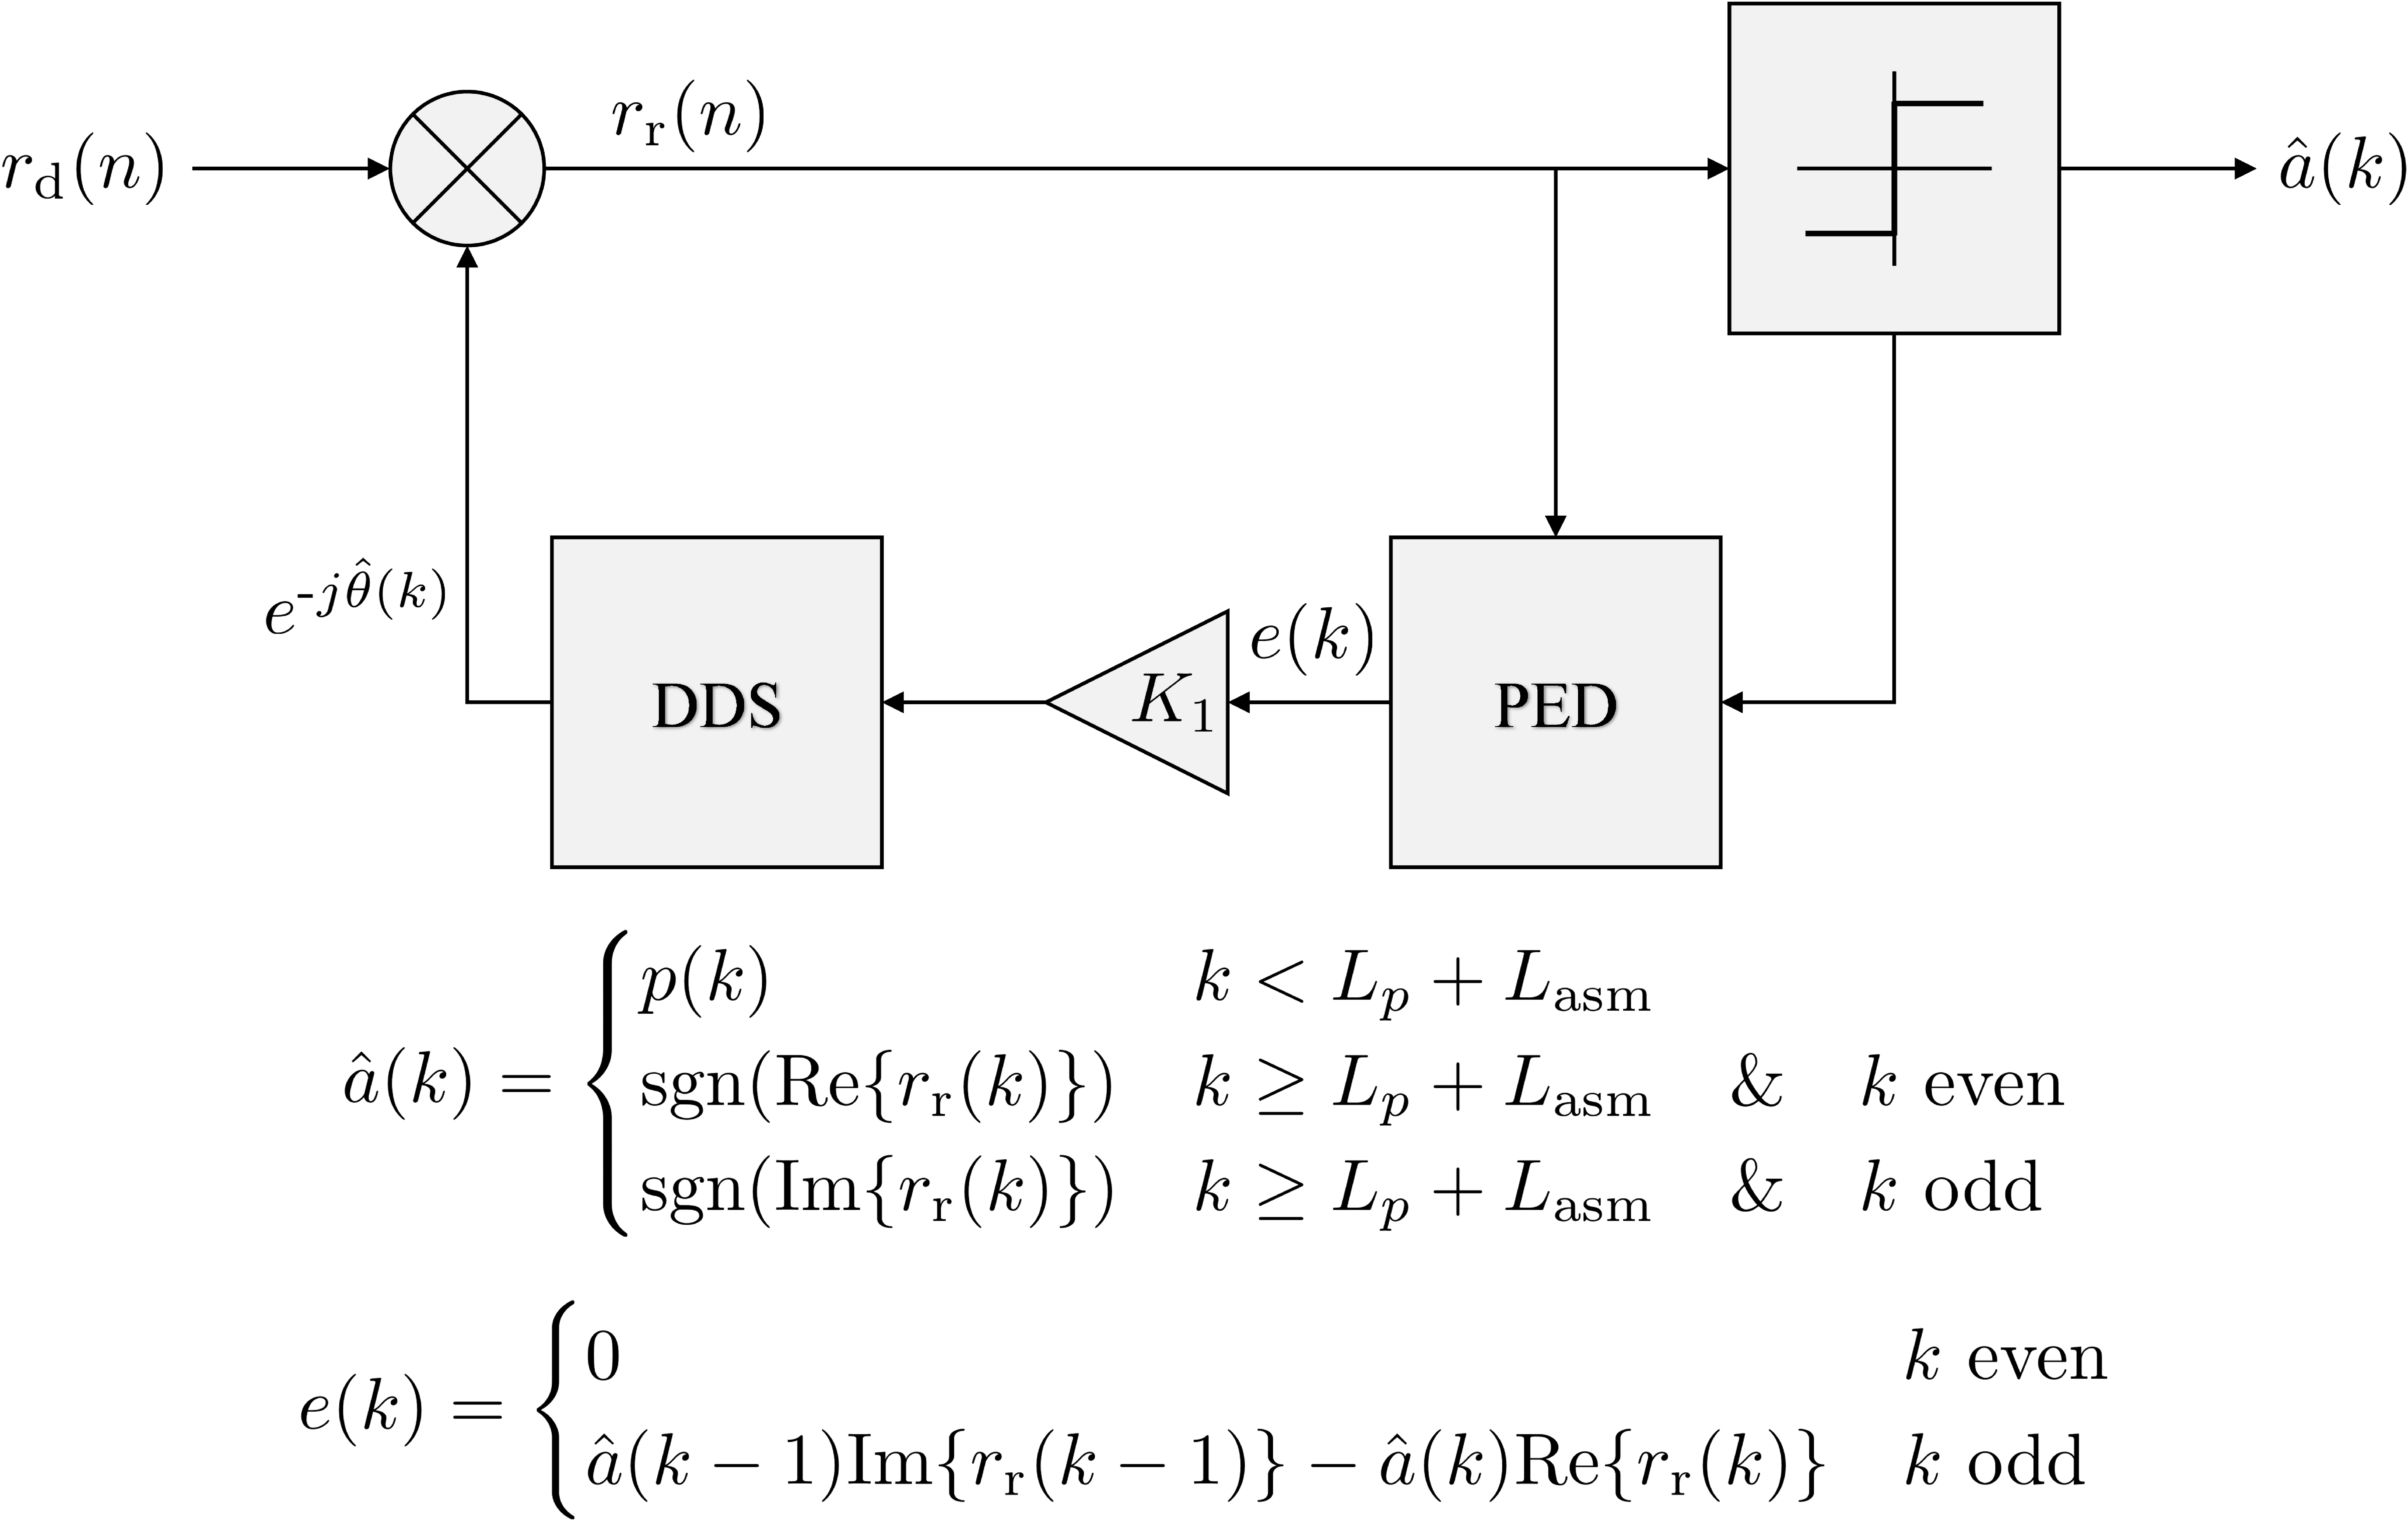
\includegraphics[width=9.11in/100*55]{figures/systemOverview/OQPSK.pdf}
	\caption{Offset Quadriture Phase Shift Keying symbol by symbol detector.}
	\label{fig:OQPSK}
\end{figure}

A Phase Lock Loop (PLL) is needed in the OQPSK detector to track out residual frequency offset.
The residual frequency offset results from a frequency offset estimation error.
Equalizers mitigate the effects of phase offset, timing offset, and ISI because all of these imparments form the  composite channel seen by the equalizer.
A frequency offset is different, and cannot be mitigated by the equalizer alone.
The PLL tracks out the residual frequency offset using a feedback control loop.

Implementing a PLL may not seem feasible in GPUs because the feedback loop cannot be parallelized.
But the PAQ system processes $3104$ packets of data simultaneously in parallel.
Running the PLL and detector serially through a full packet of samples is relatively fast because each iteration requires only $10$ floating point operations and a few logic decisions.
%
%\section{Detailed Description of Data-aided Equalizers}
%\label{sec:equalizer_eq}
%This thesis examines the GPU implementation of the five equalizer filters.
%While the performance and GPU implementation is interesting, this thesis makes no claim of theoretically expanding understanding of equalizers.
%The data-aided equalizers studied in this thesis are:
%\begin{itemize}
%\item zero-forcing (ZF) equalizer
%\item minimum mean square Error (MMSE) equalizer
%\item MMSE-initialized constant modulus algorithm (CMA) equalizer
%\item frequency domain equalizer one (FDE1)
%\item frequency domain equalizer Two (FDE2).
%\end{itemize}
%The final equations for ZF and MMSE FIR equalizer filters are very similar but differ in formulation.
%The equations for FDE1 and FDE2 are also very similar but differ by one subtle difference.
%The CMA FIR equalizer filter is computed using a steepest decent algorithm initialized by MMSE.
%More CMA iterations lead to lower BER but ZF, MMSE, FDE1 and FDE2 only require one iteration.
%The equations explained in this section will be referenced heavily in Chapter \ref{chap:equalizers_in_gpus}.
%
%\subsection{Zero-Forcing and Minimum Mean Square Error Equalizers}
%\label{sec:ZFnMMSE}
%The ZF and MMSE equalizers are treated together here because they have many common features.
%Both equalizers are found by solving linear equations
%\begin{equation}
%\mathbf{A}\mathbf{c} = \mathbf{b}
%\end{equation}
%where $\mathbf{c}$ is a vector of desired equalizer coefficients
%and the square matrix $\mathbf{A}$ and vector $\mathbf{b}$ are known.
%It will be shown that the only difference between ZF and MMSE lies in the matrix $\mathbf{A}$.
%
%\subsubsection{Zero-Forcing}
%\label{sec:zero-forcing}
%The ZF equalizer is an FIR filter defined by the coefficients
%\begin{equation}
%\begin{matrix}
%c_\text{ZF}(-L_1) & \cdots & c_\text{ZF}(0) & \cdots & c_\text{ZF}(L_2).
%\end{matrix}
%\end{equation}
%The filter coefficients are the solution to the matrix vector equation \cite[eq. (311)]{PAQ-phase1}
%\begin{equation}
%\mathbf{R}_{\hat{h}} \mathbf{c}_\text{ZF} = \hat{\mathbf{h}}_{n_0}
%\label{eq:start_here_ZF}
%\end{equation}
%where
%\begin{equation}
%\mathbf{c}_\text{ZF} = 
%\begin{bmatrix}
%c_\text{ZF}(-L_1) \\ \vdots \\ c_\text{ZF}(0) \\ \vdots \\ c_\text{ZF}(L_2)
%\end{bmatrix},
%\end{equation}
%\begin{equation}
%\mathbf{R}_{\hat{h}} = 
%\mathbf{H}^\dagger \mathbf{H} = 
%		\begin{bmatrix}
%		r_{\hat{h}}(0)			& r^\ast_{\hat{h}}(1)	& \cdots 	& r^\ast_{\hat{h}}(L_{eq}-1)  	\\
%		r_{\hat{h}}(1) 			& r_{\hat{h}}(0)		& \cdots 	& r^\ast_{\hat{h}}(L_{eq}-2)  	\\
%		\vdots	 				& \vdots				& \ddots 	&  								\\
%		r_{\hat{h}}(L_{eq}-1)	& r_{\hat{h}}(L_{eq}-2)	& \cdots	& r_{\hat{h}}(0)  			
%	\end{bmatrix}
%	\label{eq:R_h}
%\end{equation}
%and
%\begin{equation}
%\hat{\mathbf{h}}_{n_0} = \mathbf{H}^\dagger \mathbf{u}_{n_0} = 
%\begin{bmatrix} \hat{h}^\ast(L_1) \\ \vdots \\ \hat{h}^\ast(0) \\ \vdots \\ \hat{h}^\ast(-L_2)  \end{bmatrix},
%\label{eq:h_no}
%\end{equation}
%where
%\begin{equation}
%r_{\hat{h}}(k) = \sum_{n=-N_1}^{N_2} \hat{h}(n) \hat{h}^\ast(n-k),
%\label{eq:sample_autocorrelation_ZF}
%\end{equation}
%\begin{equation}
%\mathbf{u}_{n_0} = \begin{bmatrix} 0 \\ \vdots \\ 0 \\ 1 \\ 0 \\ \vdots \\ 0 \end{bmatrix}
%	\begin{matrix*}[l] \left. \vphantom{\begin{matrix} 0 \\ \vdots \\ 0 \end{matrix}} \right\}
%		\text{$n_0-1$ zeros}
%		\\ \\
%		\left. \vphantom{\begin{matrix} 0 \\ \vdots \\ 0 \end{matrix}} \right\}
%		\text{$N_1+N_2+L_1+L_2-n_0+1$ zeros}
%		\end{matrix*},
%		\label{eq:un0_ZF}
%\end{equation}
%$n_0 = N_1+L_1+1$ and
%\begin{equation} 
%\mathbf{H} = 
%		\begin{bmatrix}
%		\hat{h}(-N_1)		&  				& 		 	&  					\\
%		\hat{h}(-N_1+1) 	& \hat{h}(-N_1)	& 		 	&  					\\
%		\vdots	 			& \vdots		& \ddots 	&  					\\
%		\hat{h}(N_2)		& \hat{h}(N_2-1)&  			& \hat{h}(-N_1)  	\\
%		 					& \hat{h}(N_2) 	&  			& \hat{h}(-N_1+1) 	\\
%		 					&  	   			&  			& \vdots			\\
%		 					&  	   			&  			& \hat{h}(N_2)		\\
%	\end{bmatrix}.
%\end{equation}
%
%The $(L_\text{EQ} \times L_\text{EQ})$ auto-correlation matrix $\mathbf{R}_{\hat{h}}$ comprises the sample auto-correlation $r_{\hat{h}}(k)$.
%Building $\mathbf{R}_{\hat{h}}$ using $r_{\hat{h}}(k)$ eliminates the need for the matrix matrix multiplication $\mathbf{H}^\dagger \mathbf{H}$.
%Note that the sample auto-correlation $r_{\hat{h}}(k)$ only has support on $-(L_{ch}-1) \leq k \leq L_{ch}-1$, making the auto-correlation matrix $\mathbf{R}_{\hat{h}}$ sparse or $63\%$ zero.
%
%\subsubsection{MMSE Equalizer}
%The MMSE equalizer is an FIR filter defined by the coefficients
%\begin{equation}
%\begin{matrix}
%c_\text{MMSE}(-L_1) & \cdots & c_\text{MMSE}(0) & \cdots & c_\text{MMSE}(L_2).
%\end{matrix}
%\end{equation}
%The filter coefficients are the solution to the matrix vector equation \cite[eq. (330) and (333)]{PAQ-phase1}
%\begin{equation}
%\mathbf{R} \mathbf{c}_\text{MMSE} = \mathbf{g}^\dagger
%\label{eq:start_here_MMSE}
%\end{equation}
%where
%\begin{equation}
%\mathbf{c}_\text{MMSE} = 
%\begin{bmatrix}
%c_\text{MMSE}(-L_1) \\ \vdots \\ c_\text{MMSE}(0) \\ \vdots \\ c_\text{MMSE}(L_2)
%\end{bmatrix},
%\end{equation}
%\begin{equation}
%\mathbf{R} = 
%\mathbf{G}\mathbf{G}^\dagger + 2\hat{\sigma}^2_w \mathbf{I}_{L_1+L_2+1} = 
%\begin{bmatrix}
%r_{h}(0) + 2\hat{\sigma}^2_w	& r^\ast_{h}(1)							& \cdots 	& r^\ast_{h}(L_{eq}-1) 	\\
%r_{h}(1) 						& r_{h}(0) + 2\hat{\sigma}^2_w& \cdots 	& r^\ast_{h}(L_{eq}-2)  			\\
%\vdots	 						& \vdots								& \ddots 	&  						\\
%r_{h}(L_{eq}-1)					& r_{h}(L_{eq}-2)						& \cdots	& r_{h}(0)+2\hat{\sigma}^2_w  
%\end{bmatrix}
%\label{eq:R}
%\end{equation}
%and
%\begin{equation}
%\mathbf{g}^\dagger = \hat{\mathbf{h}}_{n0} = \begin{bmatrix} \hat{h}^\ast(L_1) \\ \vdots \\ \hat{h}^\ast(0) \\ \vdots \\ \hat{h}^\ast(-L_2)  \end{bmatrix},
%\label{eq:g_dagger_h_n0}
%\end{equation}
%where
%\begin{equation}
%r_{\hat{h}}(k) = \sum_{n=-N_1}^{N_2} \hat{h}(n) \hat{h}^\ast(n-k)
%\label{eq:sample_autocorrelation_MMSE}
%\end{equation}
%and
%\begin{equation}
%\mathbf{G} = 
%		\begin{bmatrix}
%		\hat{h}(N_2)		& \cdots		& \hat{h}(-N_1) 	&  				  \\
%							& \hat{h}(N_2)	& \cdots 			& \hat{h}(-N_1)	  \\
%				 			& 				& \ddots 			&  				& \ddots	  \\
%		 					&  	   			&  					& \hat{h}(N_2)	& \cdots	& \hat{h}(-N_1)	\\
%	\end{bmatrix}.
%\end{equation}
%
%The $(L_\text{EQ} \times L_\text{EQ})$ auto-correlation matrix $\mathbf{R}$ comprises the sample auto-correlation $r_{\hat{h}}(k)$ and the noise variance estimate $\hat{\sigma}^2_w$.
%Building $\mathbf{R}$ using $r_{\hat{h}}(k)$ and $\hat{\sigma}^2_w$ eliminates the need for the matrix matrix multiplication $\mathbf{G}\mathbf{G}^\dagger$.
%Note that the sample auto-correlation $r_{\hat{h}}(k)$ only has support on $-(L_{ch}-1) \leq k \leq L_{ch}-1$ and the addition of $\hat{\sigma}^2_w$ does not increase that support, making the auto-correlation matrix $\mathbf{R}$ sparse or $63\%$ zero.
%
%%where $\mathbf{I}_{L_1+L_2+1}$ is the $(L_1+L_2+1)\times(L_1+L_2+1)$ identity matrix,
%%$\hat{\sigma}^2_w$ is the estimated noise variance, $\mathbf{G}$ is the $(L_1+L_2+1)\times(N_1+N_2+L_1+L_2+1)$ matrix given by
%%\begin{equation}
%%\mathbf{G} = 
%%		\begin{bmatrix}
%%		\hat{h}(N_2)		& \cdots		& \hat{h}(-N_1) 	&  				  \\
%%							& \hat{h}(N_2)	& \cdots 			& \hat{h}(-N_1)	  \\
%%				 			& 				& \ddots 			&  				& \ddots	  \\
%%		 					&  	   			&  					& \hat{h}(N_2)	& \cdots	& \hat{h}(-N_1)	\\
%%	\end{bmatrix}
%%\end{equation}
%%and $\mathbf{g}^\dagger$ is the $(L_1+L_2+1)\times1$ vector given by
%%\begin{equation}
%%\mathbf{g}^\dagger = \hat{\mathbf{h}}_{n0} = \begin{bmatrix} \hat{h}^\ast(L_1) \\ \vdots \\ \hat{h}^\ast(0) \\ \vdots \\ \hat{h}^\ast(-L_2)  \end{bmatrix}.
%%%\begin{bmatrix} \hat{h}(L_1) \cdots \hat{h}(-L_2) \end{bmatrix}.
%%\label{eq:g_dagger_h_n0}
%%\end{equation}
%%
%%Computing $\mathbf{c}_\text{MMSE}$ can be simplified by noticing that $\mathbf{g}^\dagger = \hat{\mathbf{h}}_{n_0}$, $\mathbf{G}\mathbf{G}^\dagger = \mathbf{R}_{\hat{h}}$ in Equation \eqref{eq:R_h}.
%%To further simplify MMSE, twice the estimated noise variance is added down the diagonal of the channel estimate auto-correlation matrix
%%\begin{equation}
%%\mathbf{R} = 
%%\mathbf{R}_{\hat{h}} + 2\hat{\sigma^2_w} \mathbf{I}_{L_1+L_2+1} = 
%%		\begin{bmatrix}
%%		r_{h}(0) + 2\hat{\sigma^2_w}	& r^\ast_{h}(1)							& \cdots 	& r^\ast_{h}(L_{eq}-1)  	\\
%%		r_{h}(1) 						& r_{h}(0) + 2\hat{\sigma^2_w}& \cdots 	& r^\ast_{h}(L_{eq}-2)  				\\
%%		\vdots	 						& \vdots								& \ddots 	&  							\\
%%		r_{h}(L_{eq}-1)					& r_{h}(L_{eq}-2)						& \cdots	& r_{h}(0) + 2\hat{\sigma^2_w}  			
%%	\end{bmatrix}.
%%	\label{eq:R_MMSE}
%%\end{equation}
%%By placing Equation \eqref{eq:R_MMSE} and \eqref{eq:g_dagger_h_n0} into \eqref{eq:c_MMSE_direct} results in
%%\begin{equation}
%%\mathbf{c}_\text{MMSE} = \mathbf{R}^{-1} \hat{\mathbf{h}}_{n_0}.
%%\end{equation}
%%Solving for the MMSE equalizer coefficients $\mathbf{c}_\text{MMSE}$ takes the form like the ZF equalizer coeffiencts in \eqref{eq:c_ZF_solve}
%%\begin{equation}
%%\mathbf{R}\mathbf{c}_\text{MMSE} = \hat{\mathbf{h}}_{n_0}.
%%\label{eq:c_MMSE_solve}
%%\end{equation}
%%
%%The only difference between solving for the ZF and MMSE equalizer coefficients is $\mathbf{R}$ and $\mathbf{R}_{\hat{h}}$. 
%%The MMSE equalizer coefficients $\mathbf{c}_\text{MMSE}$ uses the noise variance estimate when building $\mathbf{R}$.
%%The sparseness of $\mathbf{R}$ can also be leveraged to reduce computation drastically because
%%$\mathbf{R}$ has the same sparse properties as $\mathbf{R}_{\hat{h}}$.
%
%\subsection{The Constant Modulus Algorithm}
%\label{sec:CMA}
%The $b$th CMA equalizer is an FIR filter defined by the coefficients
%\begin{equation}
%\begin{matrix}
%c_\text{CMA}^b(-L_1) & \cdots & c_\text{CMA}^b(0) & \cdots & c_\text{CMA}^b(L_2).
%\end{matrix}
%\end{equation}
%The filter coefficients are calculated by a steepest decent algorithm 
%\begin{equation}
%\mathbf{c}_\text{CMA}^{b+1} = \mathbf{c}_\text{CMA}^{b}-\mu \nabla J
%\label{eq:steepest}
%\end{equation}
%initialized by the MMSE equalizer coefficients
%\begin{equation}
%\mathbf{c}_\text{CMA}^0 = \mathbf{c}_\text{MMSE}.
%\end{equation}
%The vector $\mathbf{J}$ is the cost function and $\nabla J$ is the cost function gradient \cite[eq. (352)]{PAQ-phase1}
%\begin{equation}
%	\nabla J = \frac{2}{L_{pkt}} \sum_{n=0}^{L_{pkt}-1}
%	\left[ \vphantom{\displaystyle\sum}  y(n) y^\ast(n) - 1 \right]
%	y(n)  \mathbf{r}^\ast(n).
%\label{eq:DelJcma-approxr}
%\end{equation}
%where
%\begin{equation}
%\mathbf{r}(n) = \begin{bmatrix} r(n+L_1) \\ \vdots \\ r(n) \\ \vdots \\ r(n-L_2) \end{bmatrix}.
%\end{equation}
%This means $\nabla J$ is defined by
%\begin{equation}
%\nabla J = \begin{bmatrix} \nabla J(-L_1) \\ \vdots \\ \nabla J(0) \\ \vdots \\ \nabla J(L_2) \end{bmatrix}.
%\end{equation}
%
%A DSP engineer could implement the steepest decent algorithm by computing the cost function gradient directly.
%The $L_{pkt}$ sample summation for $\nabla J$ in \eqref{eq:DelJcma-approxr} does not map well to GPUs.
%Chapter \ref{chap:gpu} will show how well convolution performs in GPUs.
%The computation for $\nabla J$ can be massaged and re-expressed as convolution.
%
%To begin messaging $\nabla J$, the term
%\begin{equation}
%z(n) = 	2\left[ \vphantom{\displaystyle\sum}  y(n) y^\ast(n) - 1 \right] y(n)
%\end{equation} 
%is defined to simplify the expression of $\nabla J$ to
%\begin{equation}
%	\nabla J = \frac{1}{L_{pkt}} \sum_{n=0}^{L_{pkt}-1}
%	z(n)  \mathbf{r}^\ast(n).
%\label{eq:DelJcma-midMassage}
%\end{equation}
%Expanding the expression of $\nabla J$ into vector form
%\begin{multline}
%\nabla J
%	= 
%	\frac{z(0)}{L_{pkt}}
%		\begin{bmatrix} r^\ast(L_1) \\ \vdots \\ r^\ast(0) \\ \vdots \\ r^\ast(L_2) \end{bmatrix} +
%	\frac{z(1)}{L_{pkt}}
%		\begin{bmatrix} r^\ast(1+L_1) \\ \vdots \\ r^\ast(1) \\ \vdots \\ r^\ast(1-L_2) \end{bmatrix} + \cdots
%	\frac{z(L_{pkt}-1)}{L_{pkt}}
%		\begin{bmatrix} r^\ast(L_{pkt}-1+L_1) \\ \vdots \\ r^\ast(L_{pkt}-1) \\ \vdots \\ r^\ast(L_{pkt}-1-L_2) \end{bmatrix}
%\label{eq:delJ_writeoutr}
%\end{multline}
%shows a pattern in $z(n)$ and $\mathbf{r}(n)$.
%The $k$th value of $\nabla J$ is
%\begin{equation}
%\nabla J(k) = \frac{1}{L_{pkt}} \sum^{L_{pkt}-1}_{m=0}  z(m) r^\ast(m-k), \quad -L_1 \leq k \leq L_2.
%\label{eq:delJ_direct_way}
%\end{equation}
%The summation almost looks like a convolution accept the conjugate on the element $r(n)$.
%To put the summation into the familiar convolution form, define
%\begin{equation}
%\rho(n) = r^\ast(n).
%\end{equation}
%Now
%\begin{equation}
%\nabla J(k) = \frac{1}{L_{pkt}} \sum^{L_{pkt}-1}_{m=0}  z(m) \rho(k-m).
%\label{eq:CMA_delJ_rice_reformed}
%\end{equation}
%
%Note that $z(n)$ has support on $0 \leq n \leq \Lpkt-1$ and 
%$\rho(n)$ has support on $-\Lpkt+1 \leq n \leq 0$, 
%the long result of the convolution sum $m(n)$ has support on $-\Lpkt+1 \leq n \leq \Lpkt-1$.
%Putting all the pieces together, we have
%\begin{align}
%m(n) &= \sum^{L_{pkt}-1}_{m=0} z(m) \rho(n-m) \nonumber \\
%	 &= \sum^{L_{pkt}-1}_{m=0} z(m) r^\ast(m-n)
%	 \label{eq:CMA_conv_z_rho}
%\end{align}
%Comparing Equation \eqref{eq:CMA_delJ_rice_reformed} and \eqref{eq:CMA_conv_z_rho} shows that 
%\begin{equation}
%\nabla J(k) = \frac{1}{L_{pkt}} m(k), \quad -L_1 \leq k \leq L_2.
%\label{eq:CMA_delJ_donzo}
%\end{equation}
%The values of interest are shown in Figure \ref{fig:convolutionFigureRice}.
%\begin{figure}
%	\centering\includegraphics[width=10in/100*55]{figures/eq_equations/convolutionFigureRice.pdf}
%	\caption{Diagram showing the relationships between $z(n)$, $\rho(n)$ and $m(n)$.}
%	\label{fig:convolutionFigureRice}
%\end{figure}
%
%This suggest the following matlab code for computing computing the gradient vector $\nabla J$ and implementing CMA.
%\begin{table}[h]
%\caption{CMA}
%\label{code:CMA}
%\singlespacing
%{\footnotesize
%\begin{verbatim}
% 1 c_CMA = c_MMSE;
% 2 for i = 1:its
% 3 	   yy = conv(r,c_CMA);
% 4     y = yy(L1+1:end-L2); % trim yy
% 5     z = 2*(y.*conj(y)-1).*y;
% 6     Z = fft(z,Nfft);
% 7     R = fft(conj(r(end:-1:1)),Nfft)
% 8     m = ifft(Z.*R);
% 9     delJ = m(Lpkt-L1:Lpkt+L2)/Lpkt;
%10     c_CMA = c_CMA-mu*delJ;
%11 end
%12 yy = conv(r,c_CMA);
%13 y = yy(L1+1:end-L2); % trim yy
%\end{verbatim}
%}
%\end{table}
%\doublespacing
%
%\clearpage
%\subsection{The Frequency Domain Equalizers}
%\label{sec:FDE}
%Frequency Domain Equalizer One (FDE1) and Frequency Domain Equalizer Two (FDE2) are very similar structure.
%FDE1 and FDE2 are adapted from Williams and Saquib \cite[eq. (11) and (12)]{williams2013linear} \cite{coon2006channel}.
%The frequency domain equalizers are the frequency-domain equivalent to the MMSE equalizer. 
%
%Using circular convolution analysis, frequency-domain equalization performed on a packet structure must have cyclic prefix that is longer than the channel response \cite{sari1994frequency,ng2007turbo,al2008single,proakis-salehi:2008}.
%Half of the iNET preamble is used as the cyclic prefix because it has eight repetitions of $\text{CD98}_\text{hex}$.
%Figure \ref{fig:cyclicPrefix} shows how the iNET packet is used as a cyclic prefix.
%\begin{figure}
%	\centering\includegraphics[width=9.47in/100*55]{figures/eq_equations/cyclicPrefix.pdf}
%	\caption{A diagram showing how the iNET packet is used as a cyclic prefix.}
%	\label{fig:cyclicPrefix}
%\end{figure}
%The length of the cyclic prefix is half the preamble length $L_\text{P}/2 = 128$.
%The length of the cyclic prefix is much longer than channel impulse response $L_h = 38$.
%
%
%
%\subsubsection{Frequency Domain Equalizer One}
%FDE1 is the MMSE equalizer applied in the frequency domain from \cite[eq. (11)]{williams2013linear}:
%\begin{equation}
%C_\text{FDE1}(e^{j\omega_k}) = \frac{\hat{H}^\ast(e^{j\omega_k})}  {|\hat{H}(e^{j\omega_k})|^2  +  \frac{1}{\hat{\sigma}^2_w}} \quad
%\omega_k = \frac{2\pi}{N_\text{FFT}} \;
%\text{for} \;
%k=0,1,\cdots,N_\text{FFT}-1
%\label{eq:FDE1}
%\end{equation}
%where $N_\text{FFT} = 2^u = 16{,}384$ where $u = {\left\lceil \log_2{\left(\Lpkt\right)}  \right\rceil} = 14$.
%The term ${\left\lceil \log_2{\left(\Lpkt\right)}  \right\rceil}$ is the ceiling of $\log_2{\left(\Lpkt\right)}$.
%The term $C_\text{FDE1}(e^{j\omega_k})$ is the frequency response of FDE1 at $\omega_k$.
%The term $\hat{H}(e^{j\omega_k})$ is the $k$th element of the length $N_\text{FFT}$ of the channel estimate $\mathbf{\hat{h}}$ frequency response at $\omega_k$.
%The term $\hat{\sigma}^2$ is the noise variance estimate, this term is completely independent of frequency because the noise is assumed to be spectrally flat or white.
%
%Equation \eqref{eq:FDE1} is straight forward to implement in GPUs.
%FDE1 is extremely fast and computationally efficient.
%
%\subsubsection{Frequency Domain Equalizer Two}
%FDE2 is also the MMSE equalizer applied in the frequency domain.
%Unlike FDE1, FDE2 incorporates knowledge of the SOQPSK-TG power spectral density.
%The frequency response of FDE2 is \cite[eq. (12)]{williams2013linear}
%\begin{equation}
%C_\text{FDE2}(e^{j\omega_k}) = \frac{\hat{H}^\ast(e^{j\omega_k})}  {|\hat{H}(e^{j\omega_k})|^2  +  \frac{\Psi(e^{j\omega_k})}{\hat{\sigma}^2_w}} \quad
%\omega_k = \frac{2\pi}{L} \;
%\text{for} \;
%k=0,1,\cdots,L-1
%\label{eq:FDE2}
%\end{equation}
%where $\Psi(e^{j\omega_k})$ is the power spectral density of SOQPSK-TG.
%Figure \ref{fig:SOQPSK_spectrum} shows $\Psi(e^{j\omega_k})$ derived using welch's method of averaging periodograms based on length $N_\text{FFT} = 16{,}384$ FFTs of SOQPSK-TG samples at a sample rate equivalent to $2$ samples/bit.
%The term $\Psi(e^{j\omega_k})$ eliminates out of band multipath that may be challenging to estimate and over come.
%\begin{figure}
%	\centering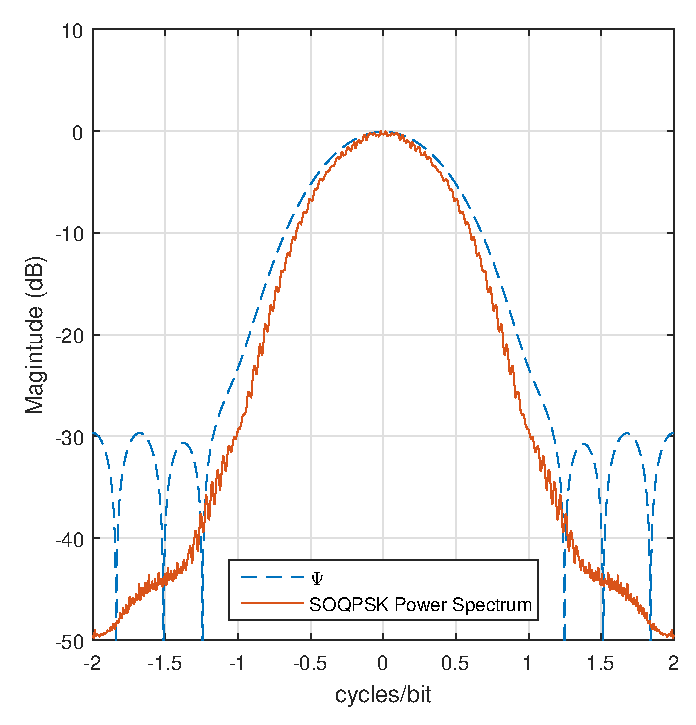
\includegraphics[width=5in]{figures/eq_equations/FDE2_spectrum_PSI.eps}
%	\caption{SOQPSK-TG power spectral density.}
%	\label{fig:SOQPSK_spectrum}
%\end{figure}
